\documentclass[11pt]{article}
\usepackage[margin=1in]{geometry}
\usepackage{graphicx,booktabs,subcaption,amsmath,microtype}
\usepackage[hidelinks]{hyperref}
\usepackage{xcolor}
\title{\textbf{A distribution-aware Bayesian logistic recognizer}\\
for real vs shuffled TCR--pMHC complexes}
\author{tcren supplementary note}
\date{}

\begin{document}
\maketitle

\section{Motivation}
The Gaussian Bayesian network of the companion note treats \emph{every} interface feature as Gaussian, which
mis-specifies the many features that are not: 15 are non-negative integer \textbf{counts} (contact and
interaction tallies, naturally Poisson) and the TCRdock \texttt{dock\_torsion} is a \textbf{circular angle}
(von Mises, wrapping $[0,2\pi)$). We replace it with a \textbf{discriminative Bayesian logistic regression},
which handles these correctly: in a discriminative model the counts are covariates that enter linearly (their
Poisson canonical form), so switching model already removes the Gaussian-on-counts mis-specification for free,
and the one representation that genuinely matters --- a circular predictor --- is entered as its von Mises
sufficient statistics $(\cos\theta,\sin\theta)$.

\section{Feature encoding}
Each feature enters the linear predictor through the canonical statistic of its natural family
(Table~\ref{tab:enc}); all columns are then standardised (train statistics only).

\begin{table}[h]\centering\small
\caption{Distribution-aware feature encoding.}\label{tab:enc}
\begin{tabular}{lll}
\toprule
family & features & encoding \\
\midrule
circular (von Mises) & \texttt{dock\_torsion} & $\to (\cos\theta,\ \sin\theta)$ \\
bounded ratio (Beta) & \texttt{chain\_balance} $\in[0,\tfrac12]$ & $\to \operatorname{logit}(2x)$ \\
counts (Poisson) & \texttt{extent}, \texttt{n\_contacts\_*}, \texttt{ct\_*} & linear (Poisson canonical) \\
unit-vector cos/sin & \texttt{dock\_\{tcr,mhc\}\_u\{y,z\}} & linear (already circular) \\
continuous & energies $F$/$\Delta F$/$e$, \texttt{burial}, \texttt{dock\_d}, \texttt{pitch}, \texttt{crossing} & linear \\
\bottomrule
\end{tabular}
\end{table}

\section{Model}
$y \sim \mathrm{Bernoulli}\!\big(\sigma(\alpha + \mathbf{z}^\top\boldsymbol\beta)\big)$ on the encoded, standardised
design $\mathbf{z}$, with weakly-informative priors $\alpha\sim\mathcal N(0,2.5)$, $\beta\sim\mathcal N(0,1)$
(a regularized-horseshoe variant is available for Bayesian sparsity). Fit with PyMC (NUTS, 2 chains). The
posterior mean is frozen into \texttt{tcren} (\texttt{tcren.recognition.\allowbreak BayesianLogisticRecognizer}). Real
(Oriented2026, $y{=}1$) vs Shuffled2026 $10\times$ decoys ($y{=}0$); 5-fold cross-validated out-of-fold
predictions give the results below. The proper encoding lifts ROC--AUC to match the random forest with a fully
interpretable linear model, above the Gaussian BN (0.865) and a plain logistic on raw features (0.870).

\begin{table}[h]\centering
\caption{Balanced cross-validated metrics (threshold at the Youden point for the point metrics).}
\label{tab:metrics}
\begin{tabular}{lr}
\toprule
metric & value \\
\midrule
ROC--AUC & 0.885 \\
PR--AUC (baseline 0.091) & 0.582 \\
balanced accuracy & 0.819 \\
$F_1$ & 0.500 \\
MCC & 0.469 \\
\bottomrule
\end{tabular}

\end{table}

\begin{figure}[h]\centering
  \begin{subcaptionbox}{ROC\label{fig:roc}}[0.42\textwidth]
    {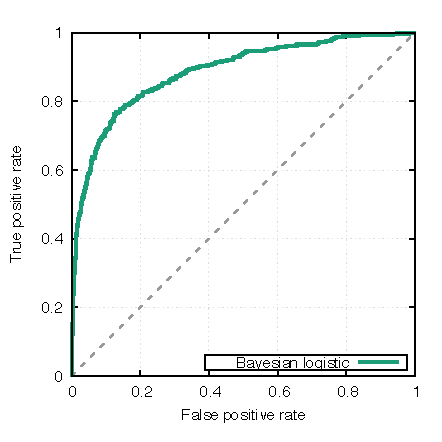
\includegraphics[width=\linewidth]{figures/roc.pdf}}
  \end{subcaptionbox}\hfill
  \begin{subcaptionbox}{Precision--recall\label{fig:pr}}[0.42\textwidth]
    {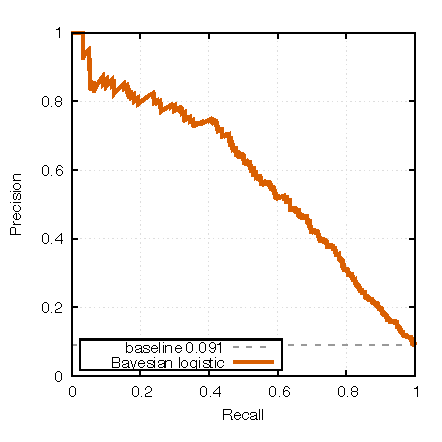
\includegraphics[width=\linewidth]{figures/pr.pdf}}
  \end{subcaptionbox}
  \caption{Real-vs-shuffled discrimination, 5-fold cross-validated out-of-fold predictions.}
\end{figure}

\begin{figure}[h]\centering
  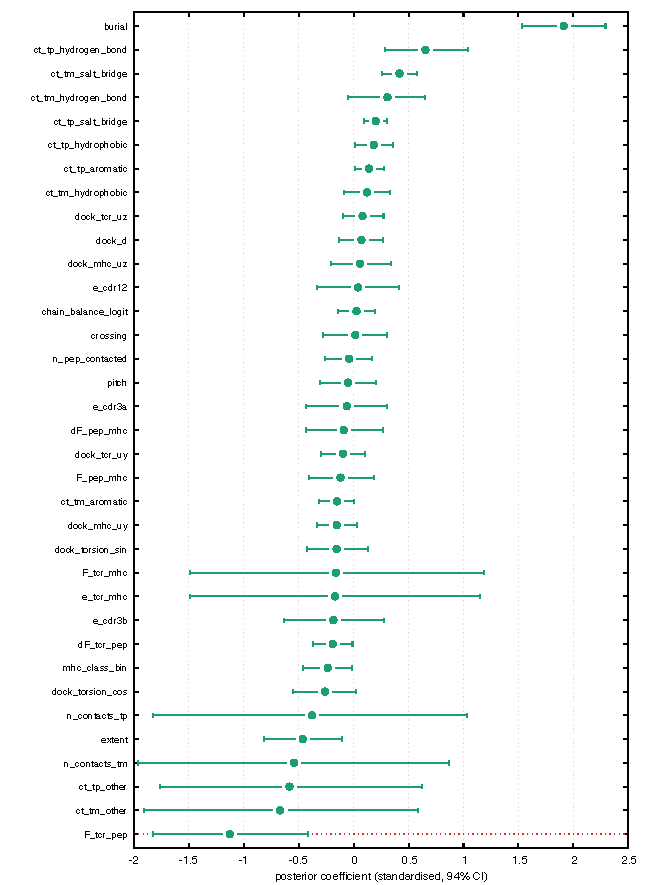
\includegraphics[height=0.82\textheight]{figures/forest.pdf}
  \caption{Posterior coefficient forest (standardised logistic weights, 94\% credible intervals; sorted). The
  two \texttt{dock\_torsion} terms are its $\cos$/$\sin$ (von Mises) components; \texttt{chain\_balance} enters
  as a logit. Coefficients whose interval excludes zero are the reliably-discriminative interface descriptors.}
\end{figure}

\end{document}
